
Dazu sollen die Befehle der Software mit einem Mikrocontroller ausgewertet werden und in, für den Drehtisch, verständliche Befehle übersetzt.
Für die Höhenverstellung des Drehtisches wird eine manuelle Steuerung im Mikrocontroller realisiert und die Endschalter so verdrahtet das sie funktionieren. \\
Der Mikrocontroller lässt sich mit mehreren Tastern bedienen und ein \Fachbegriff{LC-Display} zeigt den aktuellen Status an.\\
Der Mikrocontroller und seine Peripherie werden als \Fachbegriff{19''-Einschub} realisiert, da die Ansteuerung des Drehtisches auch als Einschub realisiert ist.\\

Der Aufbau der Arbeit gliedert sich im Wesentlichen in die Nutzung vorhandener und die Entwicklung neuer Hardware, sowie in die Entwicklung der Software für den Mikrocontroller und eine Schritt-für-Schritt Anleitung. \\
Zur Hardware gehören der 3D-Laserscanner, die Ansteuerung für den Drehtisch sowie der Drehtisch selbst, seine Spannungsversorgung, die Schrittmotoren und die Schrittmotorkarten, die Motorverkabelung, die Endschalter, sowie der Mikrocontroller, der Pegelwandler MAX232, ein LC-Display, als auch das Platinenlayout und der 19''-Einschub.\\
Zur Software gehören die 3D-Erfassungsoftware, die Entwicklungsumgebungen und die Software für den Mikrocontroller. Die Software für den Mikrocontroller deckt das Reverse-Engineering der Protokolle, deren Auswertung und Übersetzung ab; außerdem eine manuelle Ansteuerung des Drehtisches.\\
Im Anhang befindet sich eine Schritt-für-Schritt Anleitung, 3D-Modelle aufzunehmen und zu exportieren.


\begin{figure}[htb]
\centering
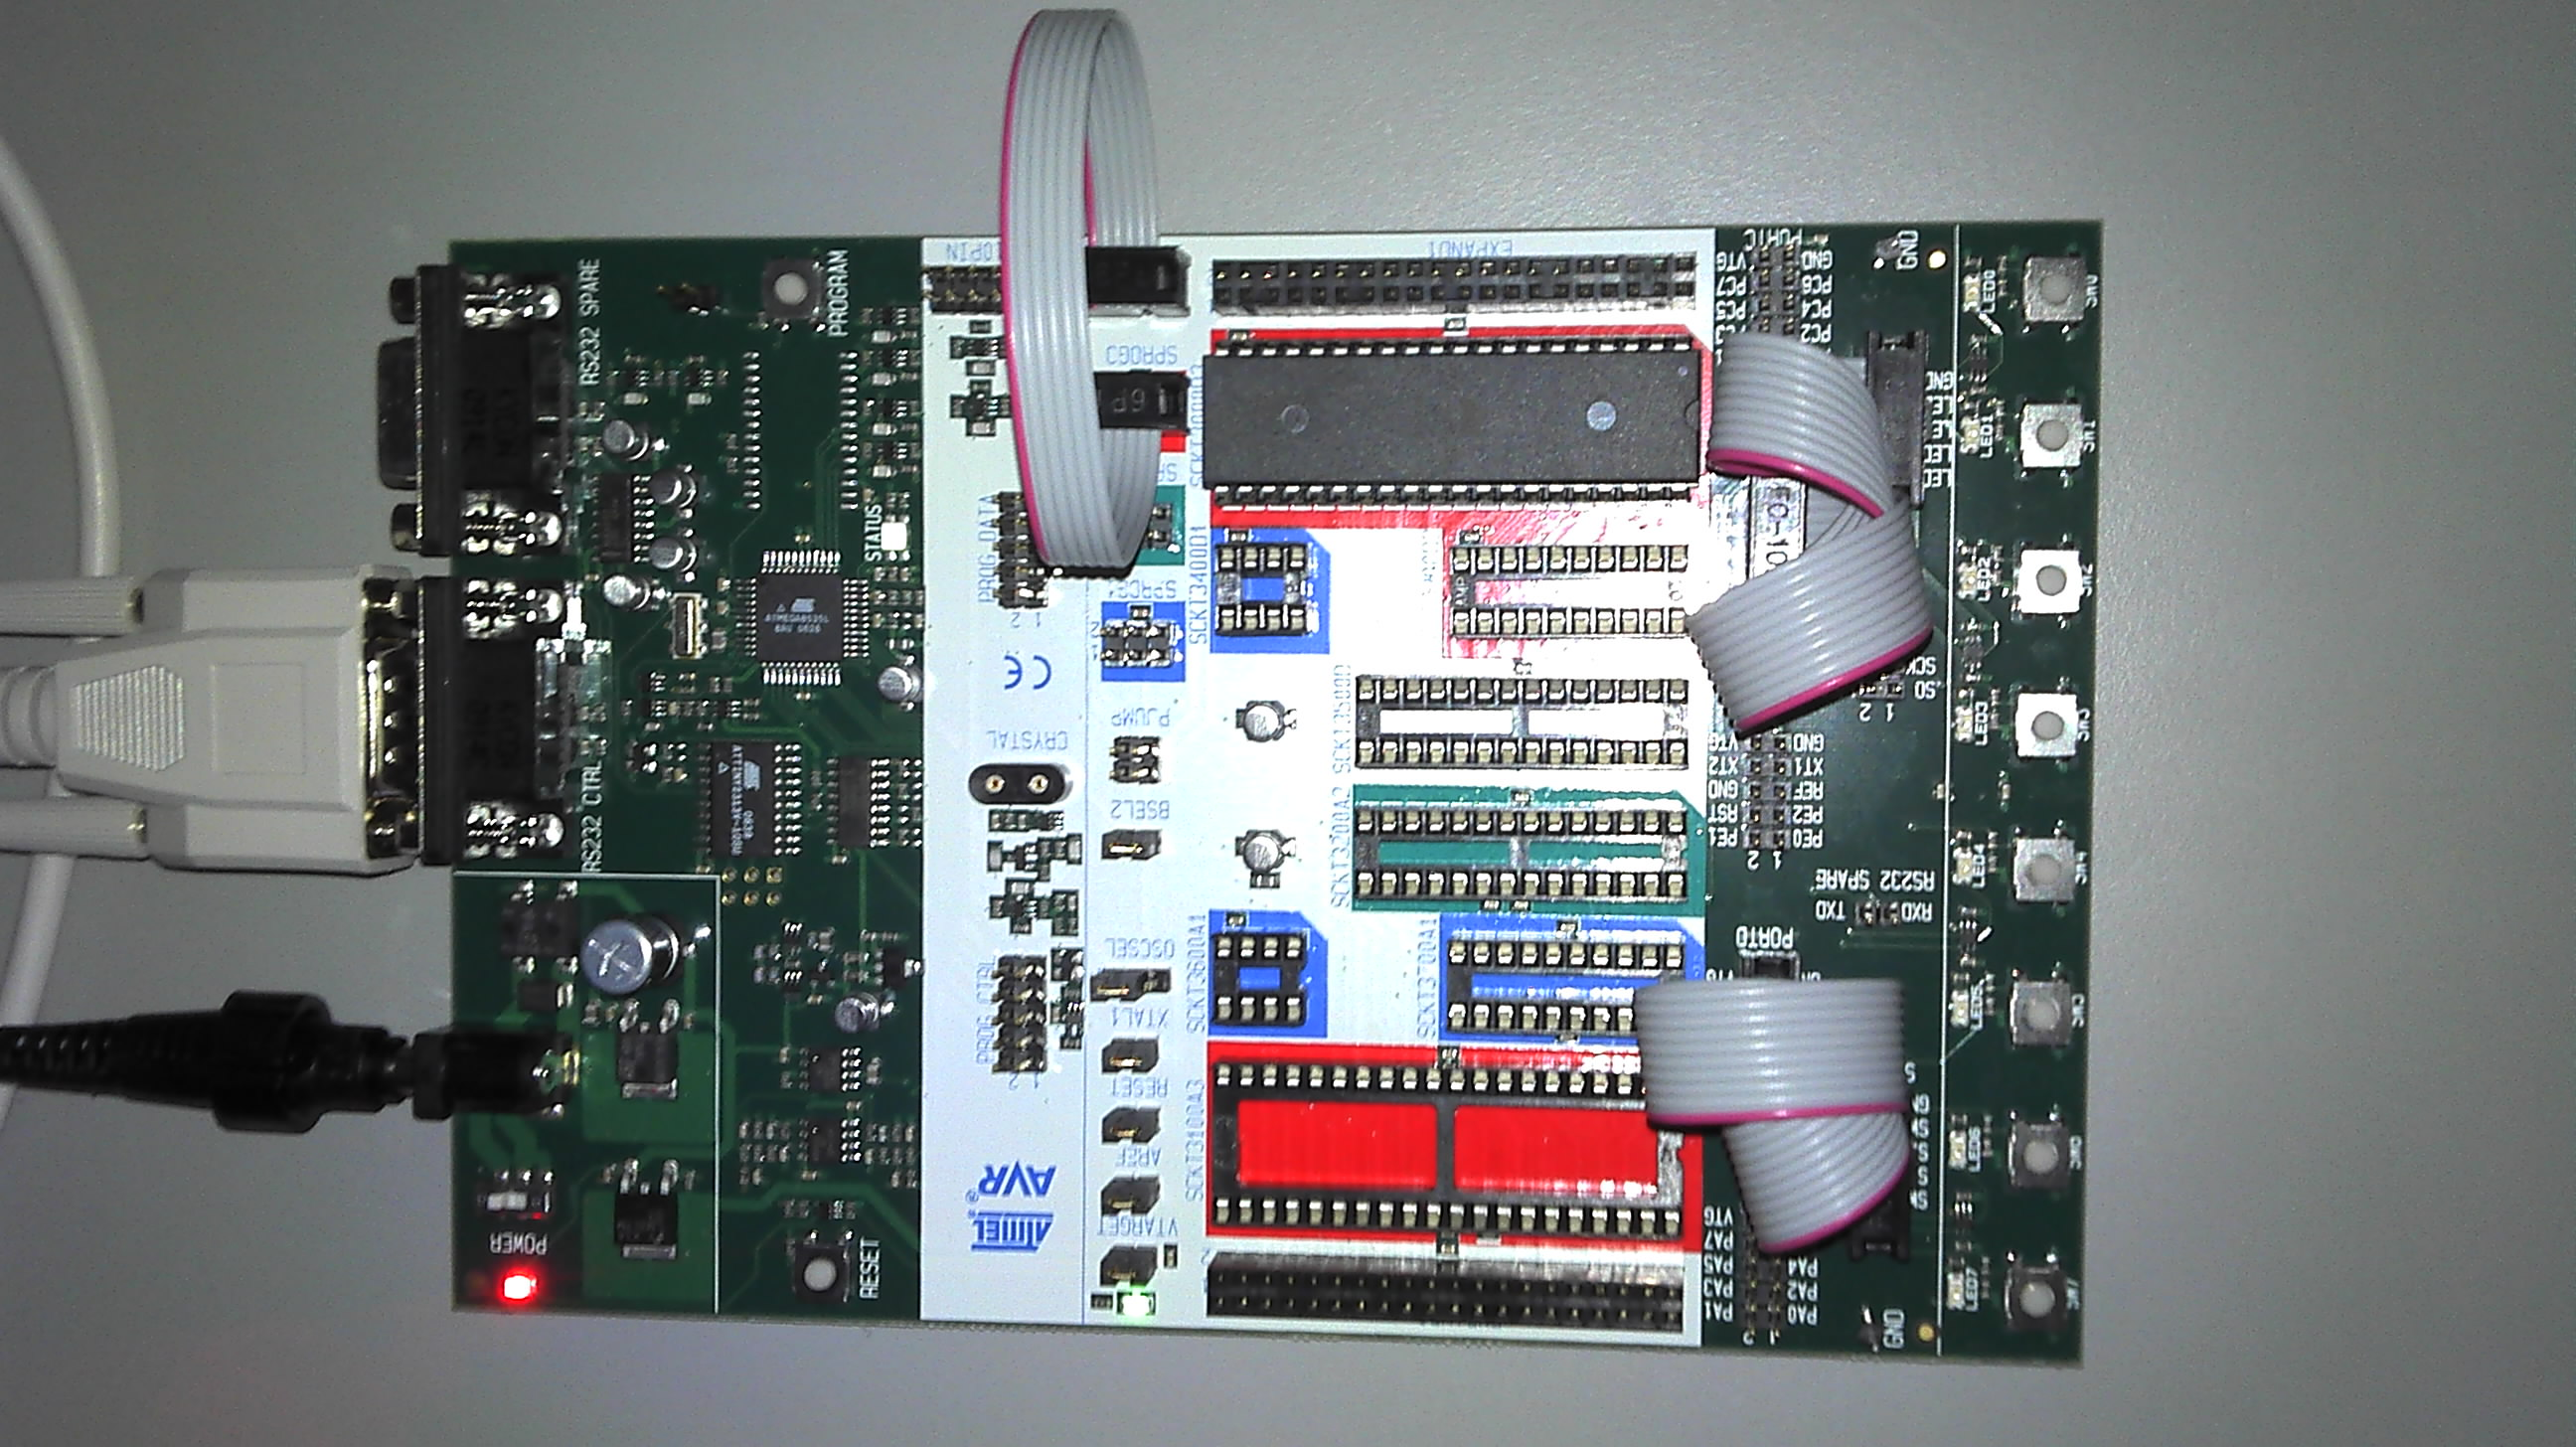
\includegraphics[width=\textwidth]{STK_500}
\caption{STK500}
\label{fig:STK500}
\end{figure}
\begin{figure}[htb]
\centering
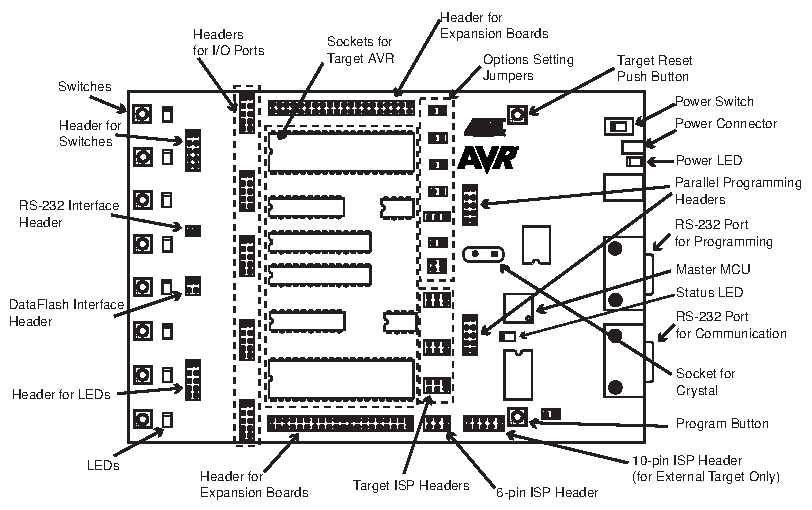
\includegraphics[width=\textwidth]{STK500_Schema}
\caption{STK500 - Schema}
\label{fig:STK500_Schema}
\end{figure}